\label{chapter:literature}

SentencePiece is an unsupervised text tokenizer and detokenizer python project, which mainly used for text generation tass.This part ia mainly based on this packet. It use a model to train what tokens are best to tokenizing a given corpus. In this part 2 different methods of tokenization in implemented. First is tokenizing words and sub-words, in this methods model looking for most repeated words and sub-words and even letter. As a result we can see almost every word in final version of chosen tokens. On the contrary the second method is just tokenizing words, this models looking for most repeated words. 
\newline
Until this part entire headline and body of each news are both covered in the corpus but from this part English values are removed from corpus so tokenization and language generation will focus on Persian. 
\newline
The corpus is shuffled 5 times and separated to train and test data. Also tokenization is applied on 4 different vocab size due to possible SentencePiece size and performance of output model is evaluated against these vocab size. In the following section, we discuss about effects of vocab size from very small value increasing to a large value.
\newline

\section{Sub-word Level}
At first i train tokenizer model on sub-words. It means model not only pays attention to words, but also pays attention to sub-words during training time. 

When the vocab size is 1000, it is too small for such a corpus and due to model type, model focuce on smaller sub-words rather than meaning full words. In final choosed-vocab, almost every character in source language exists. So when we tokenize a text there woudln't be any <unk> token and most words break into sub-words. 
\newline
As vocab size increases model learns more complicated sub-words and less meaning-less characters and sub-words. Bot the negative point is as the vocab size increases it would be harder for models to learn task and the positive point is more context will be save after tokenization.

Another point is SentencePiece can discriminate between statrting token and not starting token and ending token of a word in this mode. As we can see in \ref{fig:word2vecsubword} the are different form of one token.

\begin{figure}[h]
	\centering
	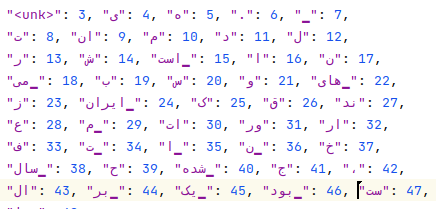
\includegraphics[width=10cm]{images/word2vec_subwordtockens.png}
	\caption{Sub-words vocab example}
	\label{fig:word2vecsubword}
\end{figure}


\section{Word Level}
In this part, i used word level tokenization, in this experience there exist <unk> token due to vocab size and model dealing with choosing best token in order to minimize <unk> token in unseen text. 
\newline
Same as previous experiment, data-set is divided into train and test set and 5 different shuffled corpus is saved, this help us to have a better evaluation on each vocab size. Four different vocab size is defined as follow: 1000, 5000, 10000, 15000. Number of <unk> token and percent of that over each corpus and vocab is reported in "report/tokenization" directory and each model and output on test set is saved in "src/tokenization/working-dir/words-out". percent of each vocab size is presented in table \ref{tbl:token-unk}.

\begin{center}
	\centering
	\begin{tabular}{|c|| c|c|c|c|c||G |} 
		\hline 
		& \multicolumn{6}{c|}{word-level} \\
		\hline
		corpus & 1 & 2 & 3 & 4 & 5 & AVG\\	
		\hline
		1000   & 0.44 & 0.44 & 0.44 & 0.43 & 0.44 & 0.44\\
		5000   & 0.20 & 0.20 & 0.20 & 0.20 & 0.20 & 0.21\\
		10000  & 0.14 & 0.14 & 0.14 & 0.14 & 0.15 & 0.15\\
		15000  & 0.12 & 0.12 & 0.12 & 0.12 & 0.14 & 0.13\\
		\hline 
	\end{tabular}
	\label{tbl:token-unk}
\end{center}

As it is illustrated in table \ref{tbl:token-unk}, number of <unk> token increase by vocab size reduction. the fewer <unk> token, the fewer information loss. On the other the larger vocab size leads into more amount of computaion for future task. As we saw it is a trade of between these to parameters, in my opinion best vocab size due to this corpus is \textbf{10000}. It has reasonable <unk> token and it may need less computation rather than 15000 vocab size.
\newline
After tokenizing corpus in word level, we can see <unk> tokens besides tokens which exist in vocabulary. In this project <unk> token id is equal to 3. Many <unk> token can be seen in tokenized validation set (Figure \ref{fig:unkrep}).

\begin{figure}[h]
	\centering
	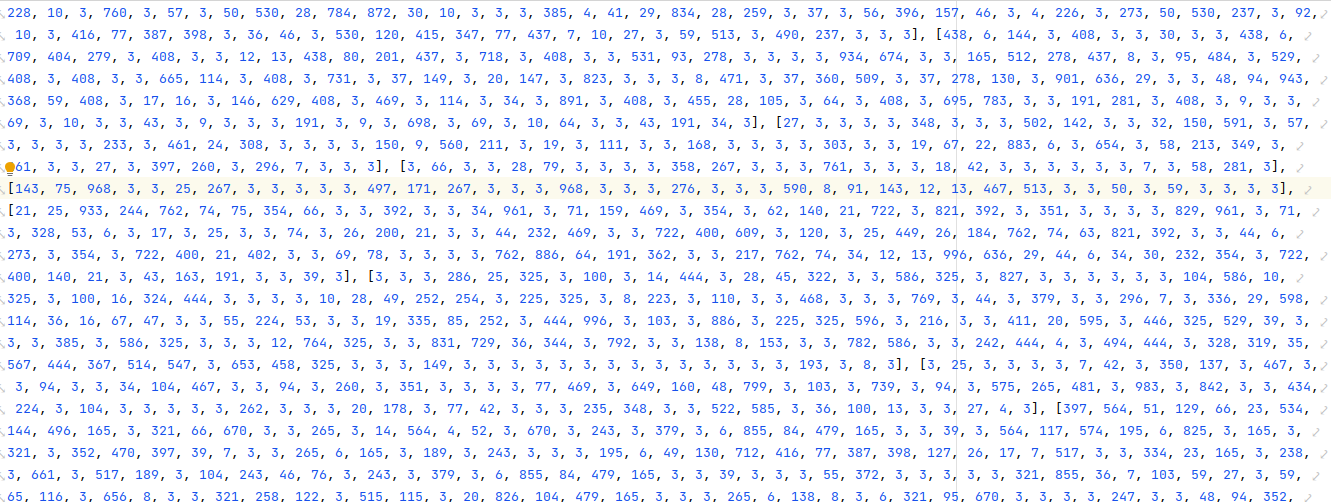
\includegraphics[width=15cm]{images/unkrep.png}
	\caption{Tokenized Corpus}
	\label{fig:unkrep}
\end{figure}
